\documentclass[french]{article}
\usepackage[T1]{fontenc}
\usepackage[utf8]{inputenc}
\usepackage{lmodern}
\usepackage[a4paper]{geometry}
\usepackage{babel}
\usepackage{graphicx}
\begin{document}
	
\begin{titlepage}
	\vspace*{\stretch{1.0}}
	\begin{center}
		\Large\textbf{Dicotomix pour le locked-in pressé}\\
		\large\textit{La team Dicotomix}
	\end{center}
	\vspace*{\stretch{2.0}}
\end{titlepage}

\begin{abstract}
	Dicotomix est un logiciel de saisie de texte mot par mot au moyen d'une navigation dans le dictionnaire. Son but principal est d'offrir une saisie rapide aux personnes en situation de handicap locomoteur lourd.
	\\
<<<<<<< HEAD
	Ce logiciel est développé par une équipe d'étudiants en première annére de master d'informatique à l'Ecole Normale Supérieure de Lyon.
=======
	Ce logiciel est développé par une équipe d'étudiants en première année de master d'informatique à l'Ecole Normale Supérieure de Lyon.
>>>>>>> 423023e137b84048317d273d363703d73c7c7ea3
\end{abstract}

\section*{Fonctionnalités}
Dicotomix permet d'écrire des phrases en français. Les accents, traits d'union et apostrophes sont disponibles. Il est également possible de rectifier une erreur en annulant la dernière opération ou en effaçant le dernier mot saisi. Dicotomix offre la possibilité de passer en mode "épellation" afin de saisir certains mots inexistants dans le dictionnaire comme les noms propres. Il est ensuite possible d'ajouter ces mots au dictionnaire. De plus, Dicotomix s'adapte à son utilisateur et lui propose en priorité les mots qu'il est le plus susceptible d'utiliser !

\section*{Protocole d'utilisation}
Commencez par choisir le mot que vous souhaitez écrire. Il ne faut surtout \textbf{pas changer de mot} une fois que vous avez commencé la recherche sous peine de ne rien trouver !
\\
Au début, Dicotomix vous propose un mot. Il s'agit d'un mot courant situé vers le milieu du dictionnaire. Vous devez ensuite indiquer au moyen des flèches droite/gauche si le mot que vous cherchez se trouve avant ou après dans l'ordre alphabétique.
\\
\begin{center}
	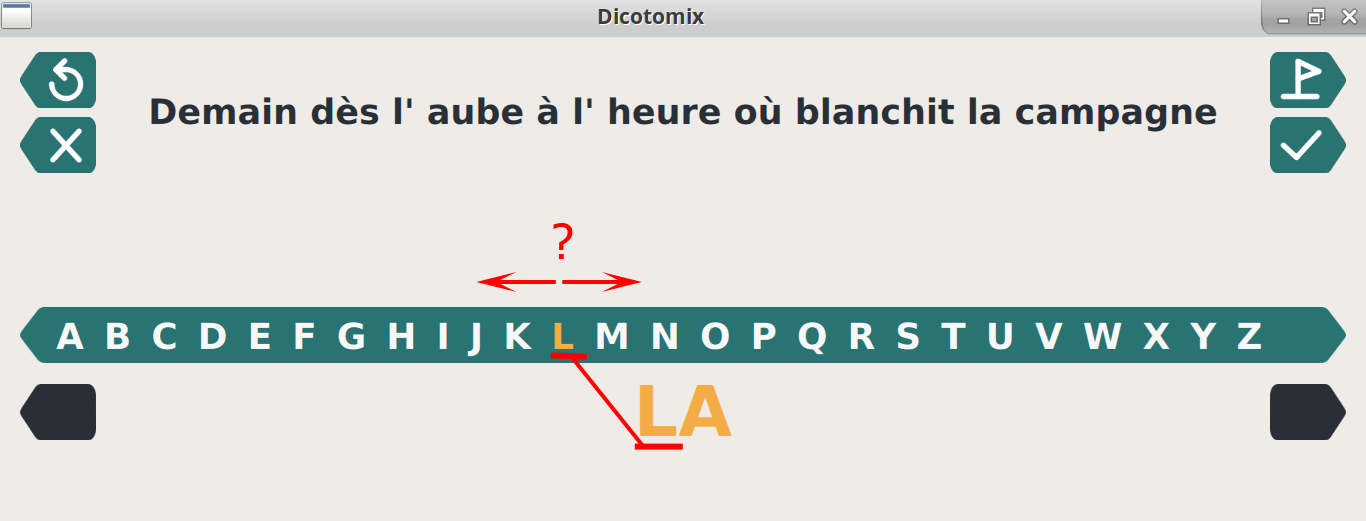
\includegraphics[scale=0.22]{ex1}
\end{center}
Une fois que le mot recherché s'affiche, validez avec la touche "Entrée".
\\
Si vous commettez une erreur lors de la recherche d'un mot, vous pouvez annuler la dernière action (ceci peut être fait plusieurs fois de suite) en appuyant sur l'icône adéquate.
\\
Au bout de plusieurs étapes, Dicotomix connaît de manière certaine le début de votre mot et l'affiche en vert. \textbf{Si le mot que vous recherchez ne commence pas par le mot vert, c'est que vous avez fait une erreur !}
\\

\begin{center}
	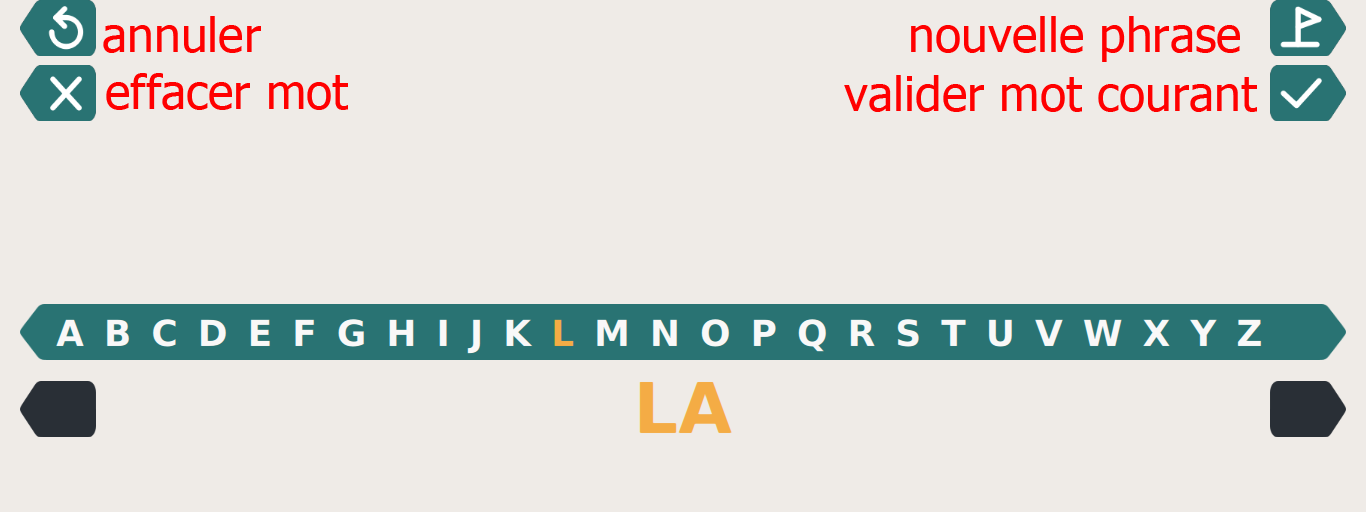
\includegraphics[scale=0.22]{vierge}
\end{center}
Notez que le tiret et l'apostrophe ne comptent pas pour l'ordre alphabétique, c'est la lettre suivante qui est prise en compte.
\\
\begin{center}
	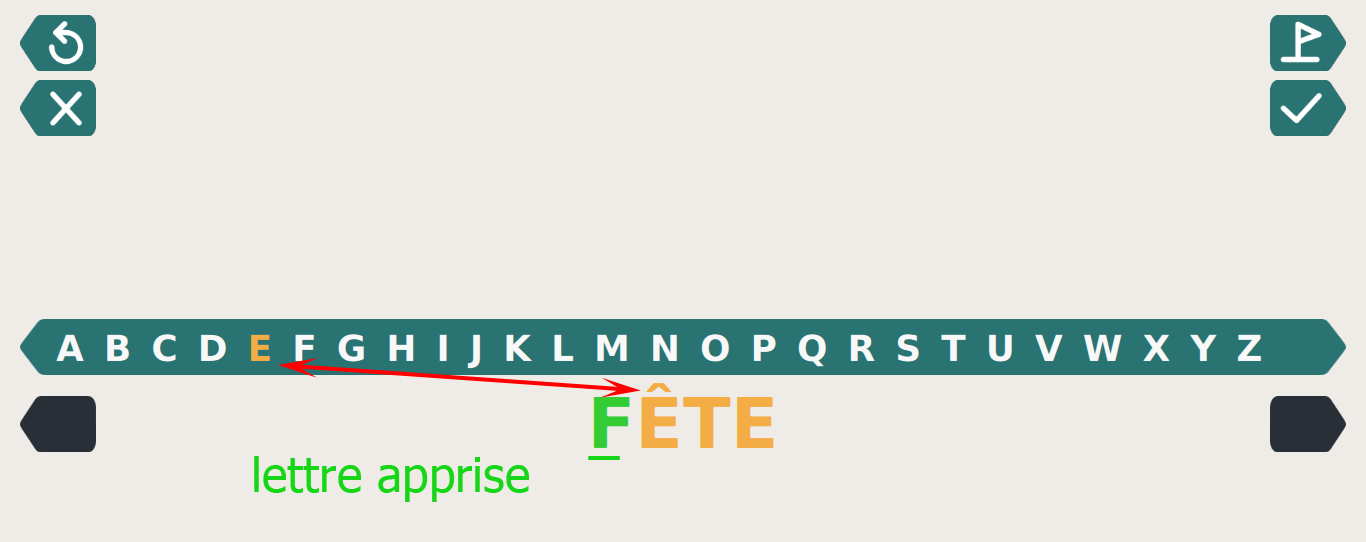
\includegraphics[scale=0.22]{encours}
\end{center}
\begin{center}
	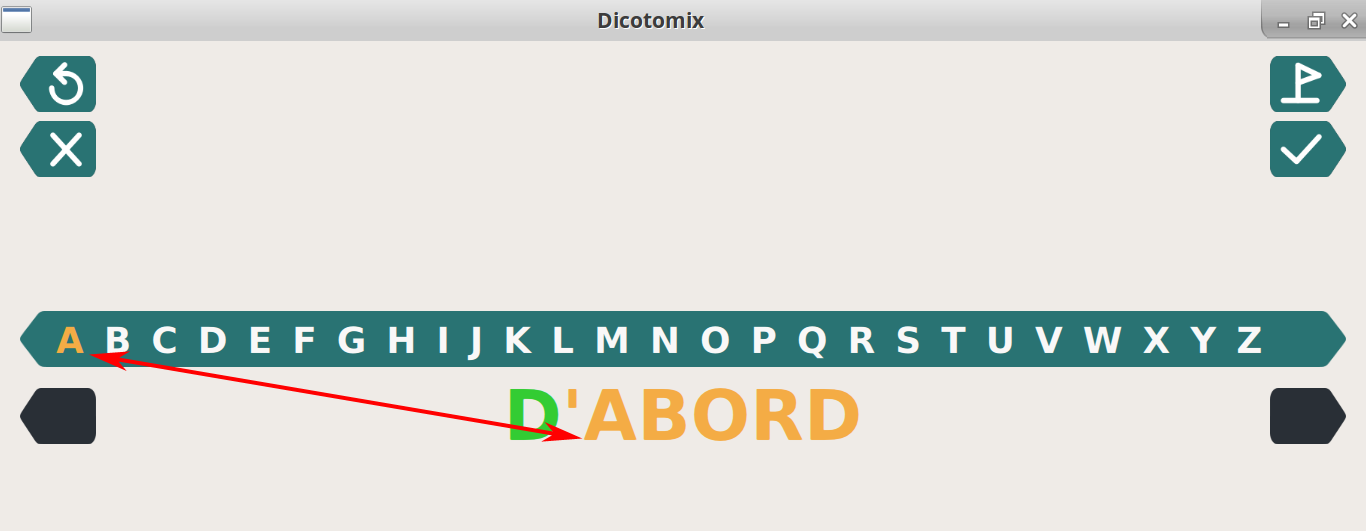
\includegraphics[scale=0.22]{apostrophe}
\end{center}

\section*{Conseils d'utilisation}
\textbf{Ne vous précipitez pas !} Il est tout à fait possible que le mot proposé commence comme le mot que vous recherchez et que le mot suivant soit très différent. Pour autant, ne vous inquiétez pas, vous avez progressé ! Il est fondamental d'accepter cette rigueur de l'ordre alphabétique afin de réussir à écrire vite grâce à Dicotomix.
\\
En cas d'erreur, il vaut souvent mieux complètement supprimer le mot plutôt que de faire plusieurs retours arrière.
\\
Quelques exemples illustrant l'ordre alphabétique utilisé :
\begin{itemize}
	\item "lequel" vient après "le"
	\item "l'" vient avant "la"
<<<<<<< HEAD
	\item En cas d'erreur, il vaut souvent mieux complètement supprimer le mot plutôt que de faire plusieurs retours arrières.
=======
	\item "porte-monnaie" vient après "portée" et avant "porter", car les tirets et les accents ne comptent pas
>>>>>>> 423023e137b84048317d273d363703d73c7c7ea3
\end{itemize}

\begin{center}
	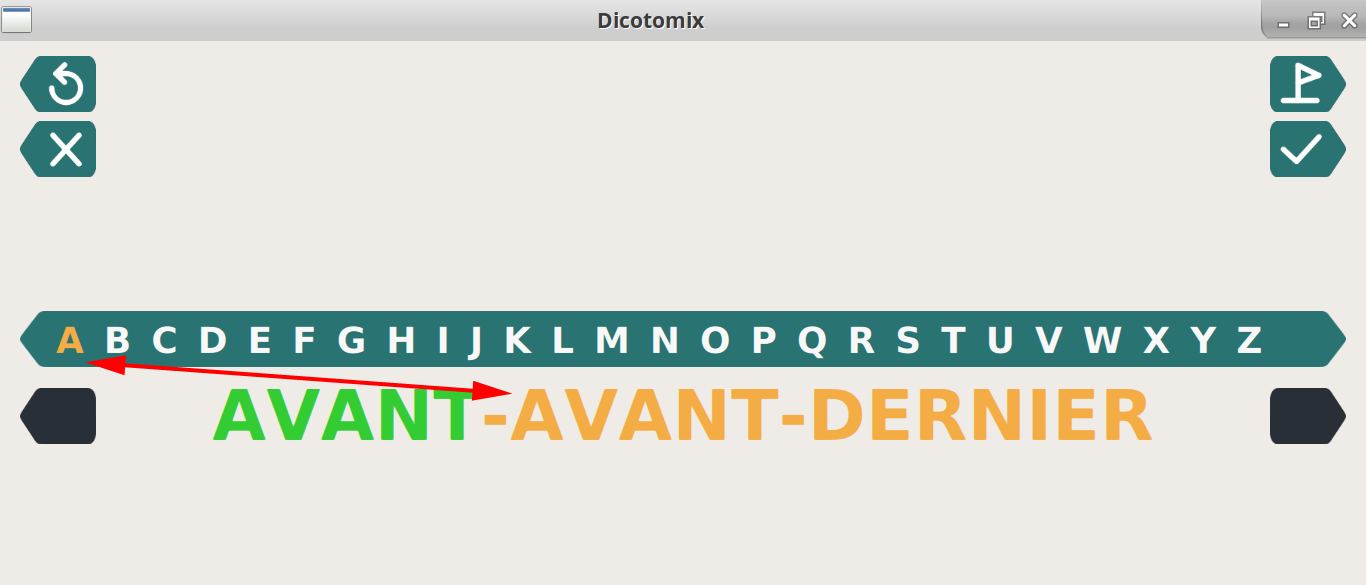
\includegraphics[scale=0.22]{tiret}
\end{center}



\end{document}
